%-----------------------------------------------------------------------------------------------
\chapter{Lokális struktúra vizsgálata}\label{sect:LocalStruct}
%-----------------------------------------------------------------------------------------------

Az illeszkedési minőség bizonyos esetekben javítható, ha figyelembe vesszük a kép lokális struktúráját.
Ez a megoldás rontja az általánosságot, mert extra megkötéseket követel meg a diszparitásra vonatkozóan.

Az alábbiakban az ilyen feltételeket és a rájuk illesztett modelleket ismertetem.
Nem minden modell került megvalósításra, néhol a vizsgálati eredményekből kiderült, nem reális vagy fölösleges részletes.

%-----------------------------------------------------------------------------------------------
\section{Modellek}\label{sect:Models}
%-----------------------------------------------------------------------------------------------

Ezen fejezet alapfeltevése, hogy a diszparitás kis régiókon belül nem változhat tetszőlegesen.
A kis régió nagyon szubjektív, jelen állás szerint kísérletileg meghatározott fogalom.
A továbbiak a kép 16 pixel széles tartományát értem ezalatt.

Már korábban is feltettük\footnote{Az ablakméret megválasztásánál}, hogy nem számítunk tetszőlegesen nagy elmozdulásokra.
A modellezés során ennél erősebb feltételek keresése volt a cél.

Két esetet vizsgáltam a féléves munka során: lineáris modell és 2 konstans szakaszból álló modell.

%-----------------------------------------------------------------------------------------------
\subsection{Lineáris modell}\label{sect:linearModel}
%-----------------------------------------------------------------------------------------------

A lineáris modell esetében az volt a feltételezés, hogy a diszparitás lineárisan változik rövid szakaszon.
Ekkor a modell \eqref{linModel} alakú.
\begin{equation}
y = a*x + b
\label{eq:linModel}
\end{equation}

Az illeszkedés hibája nyilvánvalóan igen nagy lesz, ha a diszparitásban ugrás\footnote{Ez a helyzet áll fenn például tárgyak pereménél} van a régión belül.
Kiegészíthető a modell úgy, hogy 2 egyenes szakaszt illesztünk az adatokra.
Így jóval több paraméter\footnote{Az egyenesek paraméterein túl a töréspont helyét is meg kell határozni.} meghatározása a feladat ugyan annyi bemenő adatpont használatával.
Ha ezt a problémát a régióméret növelésével próbáljuk csökkenteni, akkor pedig a modell alapfeltevése (lineáris változás) sérülhet.

Mélyebb vizsgálatnak nem vetettem alá ezt a modellt.
A jelenlegi pontossági igényeken belül még a lineáris változás is elhanyagolható kis szakaszokon.
Több mintát megvizsgálva arra jutottam, hogy a konstans modell is elegendő a feladat megoldására.

%-----------------------------------------------------------------------------------------------
\subsection{Konstans modell}\label{sect:constModel}
%-----------------------------------------------------------------------------------------------

Hasonlóan a lineáris modellhez, ebben az esetben is be meg kell engedni egy töréspontot modellben.
Így egy három paraméteres modell adódik:
\begin{itemize}[noitemsep]
\item Diszparitás a régió elején
\item Diszparitás a régió végén
\item Törés koordinátája
\end{itemize}

Még így is relatív kevés adat jut egy paraméterre (16 pixeles régióméret esetén).
A gyakorlati implementációban további optimalizálásként 2 esetet különböztetek meg.
Ha a két diszparitás paraméter eltérése igen kicsi (1-2 pixel), akkor 1 paraméteres modellt használok.

%-----------------------------------------------------------------------------------------------
\section{Illesztési módszerek}\label{sect:modelMatch}
%-----------------------------------------------------------------------------------------------

Az előző féléves munkám során a rekonstrukció eredményeként mindig a legjobb illeszkedési mutatóval rendelkező pont lett elfogadva.
A mostani módszerek ettől gyökeresen különböznek.
Az első maximumok gyakran hibás egyezés következményei, zajosak lehetnek.
Az vizualizált illeszkedési grafikonokat vizsgálva szembetűnik, hogy sok esetben az első maximum ugyan hibás, de a helyes eredmény is detektálható lenne az adatokból.
Itt jön a képbe ezen fejezet tárgya: a lokális környezet.
Ha nem csak az első maximumot tároljuk, hanem az első néhányat, a szomszédos pontok diszparitása alapján kiválaszthatjuk a legvalószínűbb egyezést közülük.

Ezt a választást segítik a feljebb vázolt modellek.
Alább pedig két lehetőséget mutatok be a paraméterek meghatározására.

%-----------------------------------------------------------------------------------------------
\subsection{Kumulált korreláció}\label{sect:CumCorr}
%-----------------------------------------------------------------------------------------------

Az diszparitás meghatározásánál az illeszkedési függvény maximumhelyei közül kell választanunk.
Általában a legnagyobb értékű maximumhely adja a helyes eredményt, ám vannak kivételek.
A \figref{matchResult} ábra egy lokális régió pixeleire kiszámolt illeszkedési függvényeket mutatja.
Kék sáv jelöli az első maximumot, fekete sávok a többi lokális maximumot. 
\begin{wrapfigure}{l}{0.35\textwidth}
	\centering
	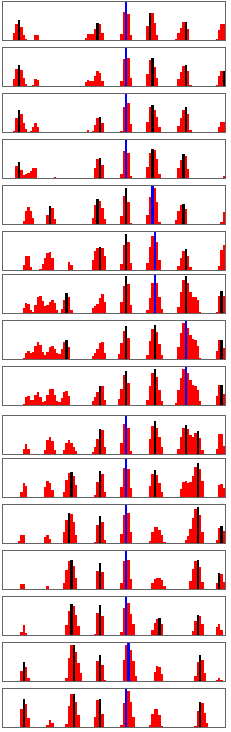
\includegraphics[width=0.35\textwidth]{figures/matchresult.png}
	\caption{Illeszkedési függvények}
	\label{fig:matchResult}
\end{wrapfigure}
Az ábrázolt régió egy sík felületet ábrázol, tehát konstans diszparitást kellene látnunk.
Az ábrán megfigyelhető, hogy ha nem az első maximumot választottuk volna, a helyes eredményt is megkaphattuk volna.

A megoldandó probléma: választanunk kell a maximumok között.
Erre egy lehetséges megoldás a kumulált korreláció vizsgálata.
Lényege, hogy az egyes illeszkedési függvényeket összeadjuk, és az összegen is elvégezzük a maximumkeresést.
Ekkor kapunk néhány diszparitás értéket, ahol több adatpont is elfogadható illeszkedést mutat.
Ezeket az értékeket felhasználhatjuk, mint klaszterek.
A két legmagasabb kumulált korrelációval rendelkező klaszterközéppontot fogadjuk el, mint modell paraméterek.

Hátra van még a töréspont meghatározása.
Ehhez minden illeszkedési függvényen ki kell számolnunk a két választott klaszterközépponthoz legjobban illeszkedő maximumok hibáit.
Így kapunk 2 hiba függvényt.
Az egyik az él előtti szakaszon, a másik az él utáni szakaszon fog kis hibát mutatni.
Optimális esetben található egy pont, ahol az egyik függvény egy adott határ alá csökken, míg a másik fölé kerül.
Ez lesz a modell 3. paramétere, az él pozíciója.

A választott diszparitás pedig mindig a modell paraméterhez legközelebbi maximum: \emph{nem} helyettesítjük a klaszterközépponttal a mért értéket.

Ennek a módszernek megvannak a korlátai: nem garantált, hogy az összegzett illeszkedés maximumai a helyes eredményt adják.
Ekkor egy hamis átlagérték közé csoportosulhatnak az eredmények, aminek következtében akár még romolhat is a kapott diszparitáskép minősége.

%-----------------------------------------------------------------------------------------------
\subsection{RANSAC}\label{sect:ransac}
%-----------------------------------------------------------------------------------------------

A RANSAC algoritmus működésének leírását itt mellőzöm, működése közismert.
Munkám során az előző pont végén leírt jelenség elleni védekezésként merült fel a használata.
A véletlenszerűen választott paraméterek itt a klaszterközéppontok, amik a talált maximumok közül kerülnek ki.
Minden iterációban elvégezzük a modell hibájának számítását, majd a legjobban illeszkedőt fogadjuk el megoldásnak.